\section{Text-to-SQL AI Service Implementation}

The text-to-SQL service is a multi-agent AI system that automatically translates natural language questions into executable SQL queries. This capability enables users without SQL expertise to interact with relational databases through conversational interfaces, significantly lowering the barrier to data exploration and analytics.

\subsection{Architecture Overview}

The text-to-SQL service implements a staged processing pipeline comprising four specialized agents: the
\textit{Selector}, the \textit{Decomposer}, the \textit{Reviewer} and the \textit{Refiner}. This design philosophy---separating schema
understanding, query decomposition, and validation---improves both reliability and interpretability compared to
single-pass code generation approaches.

\subsubsection{Service Integration Model}

The text-to-SQL service is deployed as a separate microservice communicating with the Go backend via REST API endpoints. This separation of concerns provides several advantages:

\begin{itemize}
    \item \textbf{Technology independence}: The AI service runs on Python with PyTorch and LLM inference capabilities, distinct from the Go backend's performance requirements.
    \item \textbf{Independent scaling}: The AI service can scale independently based on inference load without impacting the database control plane.
    \item \textbf{Computational isolation}: Heavy LLM inference operations do not block the backend's request handling or provisioning orchestration.
    \item \textbf{Flexible LLM integration}: The service can swap LLM providers (OpenAI, local Ollama, or other APIs) without backend changes.
\end{itemize}

The backend delegates text-to-SQL requests to the service after validating user credentials and extracting the target database connection parameters. The service then executes the full agent pipeline and returns the generated SQL for backend execution.

\subsection{Multi-Agent Pipeline}

\begin{figure}[H]
    \centering
    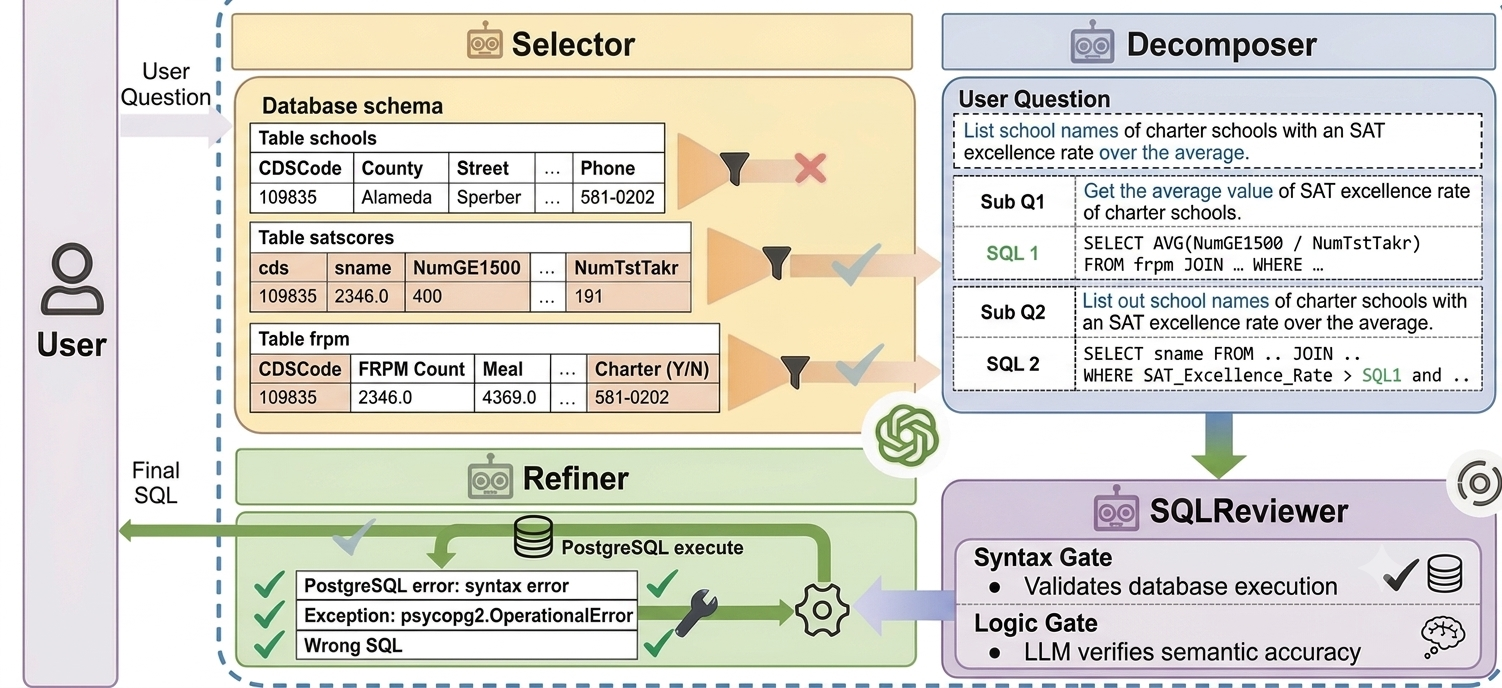
\includegraphics[width=\linewidth,height=0.9\textheight,keepaspectratio]{images/ai/text2SQL.png}
    \caption{Multi-Agent Pipeline}
    \label{fig:Multi-Agent Pipeline}
\end{figure}

\clearpage

\subsubsection{Agent 1: The Selector}

\begin{figure}[H]
    \centering
    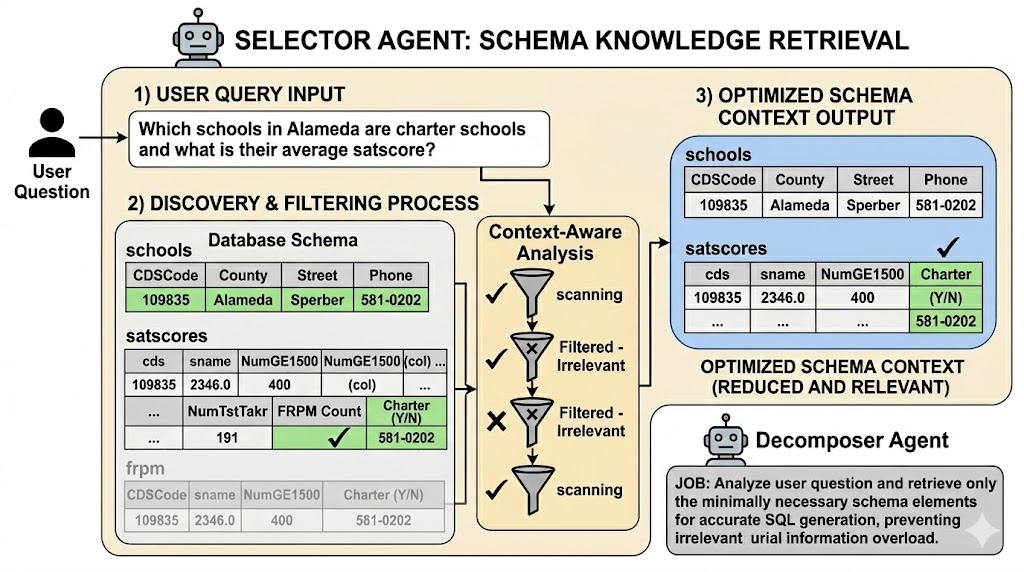
\includegraphics[width=\linewidth,height=0.9\textheight,keepaspectratio]{images/ai/Selector.jpeg}
    \caption{The Selector}
    \label{fig:The Selector}
\end{figure}

The Selector agent operates as the schema understanding component. It accepts:

\begin{itemize}
    \item The natural language question
    \item The complete database schema (table names, column names, data types, and sample values)
    \item Any user-provided hints or context
\end{itemize}

The Selector's responsibility is to identify which tables, columns, and relationships are relevant to the user's question. Rather than passing the entire schema to downstream agents (which would consume excessive token budget and introduce noise), the Selector performs semantic matching between the natural language question and schema elements. Its output is a curated subset of the schema containing only relevant entities.

This filtering step significantly improves downstream agent performance by reducing context size and eliminating schema noise that might confuse the code generation models.

\clearpage

\subsubsection{Agent 2: The Decomposer}

\begin{figure}[H]
    \centering
    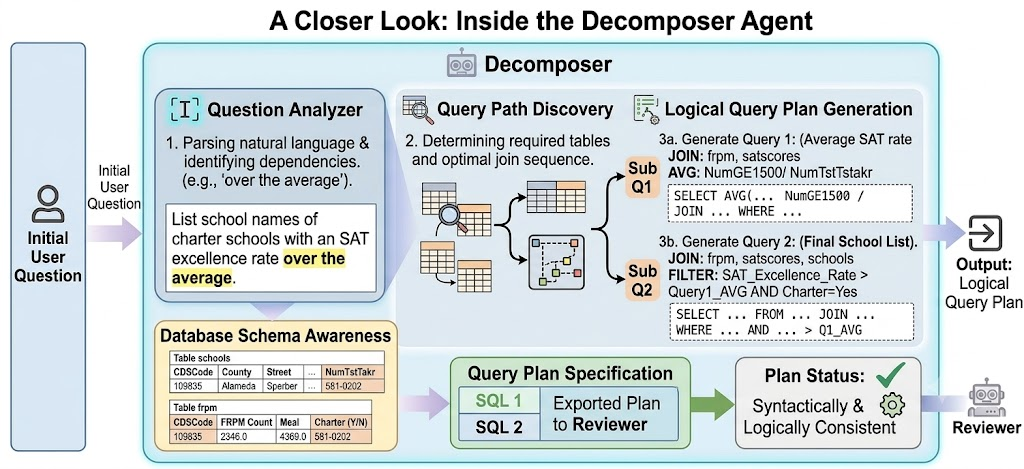
\includegraphics[width=\linewidth,height=0.9\textheight,keepaspectratio]{images/ai/Decomposer.jpeg}
    \caption{The Decomposer}
    \label{fig:The Decomposer}
\end{figure}

The Decomposer agent analyzes complex questions and breaks them into simpler sub-questions, each answerable by a focused SQL fragment or intermediate result. This staged approach follows the principle of \textit{chain-of-thought} reasoning: by expressing intermediate steps explicitly, the agent is more likely to construct logically correct queries than if attempting to generate the full SQL statement in a single pass.

The Decomposer accepts:

\begin{itemize}
    \item The original natural language question
    \item The curated schema from the Selector
    \item Optionally, a one-shot example demonstrating the decomposition format
\end{itemize}

The Decomposer outputs a structured decomposition including:

\begin{itemize}
    \item A list of sub-questions that progressively build toward the final answer
    \item For each sub-question, the intermediate SQL that would answer it
    \item A final SQL statement combining all sub-questions
\end{itemize}

For evaluation on standard text-to-SQL benchmarks (such as BIRD or Spider), the Decomposer uses dataset-specific templates optimized for each benchmark's schema patterns.

\subsubsection{Agent 3: The SQL Reviewer}

\begin{figure}[H]
    \centering
    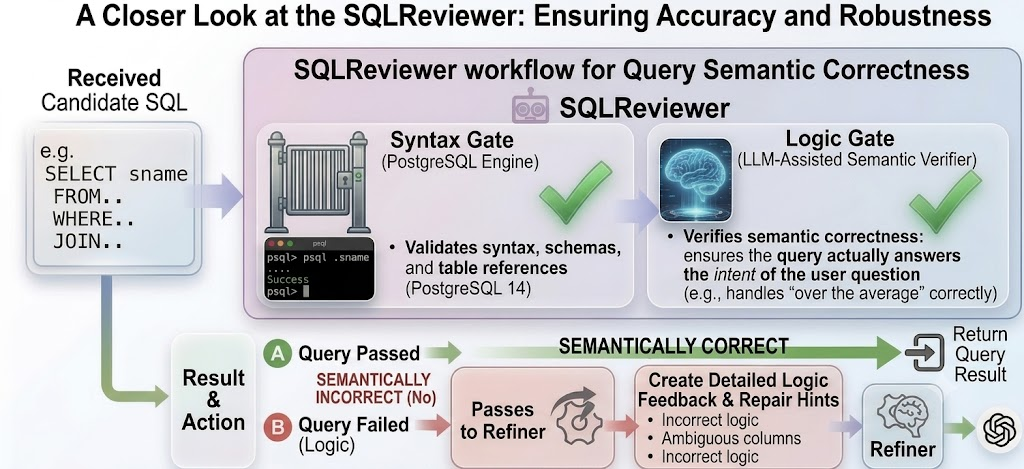
\includegraphics[width=\linewidth,height=0.9\textheight,keepaspectratio]{images/ai/Reviewer.jpeg}
    \caption{The Reviewer}
    \label{fig:The Reviewer}
\end{figure}

The SQL Reviewer agent operates as a validation-and-verification layer. It examines the generated SQL from the Decomposer, checks whether the SQL semantically answers the user query, and performs controlled execution attempts to detect runtime issues. The Reviewer analyzes:

\begin{itemize}
    \item \textbf{Syntax correctness}: Validates PostgreSQL-specific syntax (function names, operator usage, keyword combinations)
    \item \textbf{Schema consistency}: Verifies that all referenced tables, columns, and relationships exist in the provided schema
    \item \textbf{Type compatibility}: Checks type mismatches in comparisons, function arguments, and JOIN conditions
    \item \textbf{Logical coherence}: Detects suspicious patterns (e.g., JOINing unrelated tables, impossible WHERE clauses)
    \item \textbf{Query-answer alignment}: Evaluates whether the SQL is semantically consistent with the natural-language question intent
\end{itemize}

The Reviewer outputs a pass/fail decision and, if issues are detected, provides a structured report containing error messages and reasoning about why the SQL does not correctly answer the query. This early validation prevents invalid or semantically incorrect queries from being passed to later stages, improving user experience through immediate feedback.

\subsubsection{Agent 4: The Refiner}

\begin{figure}[H]
    \centering
    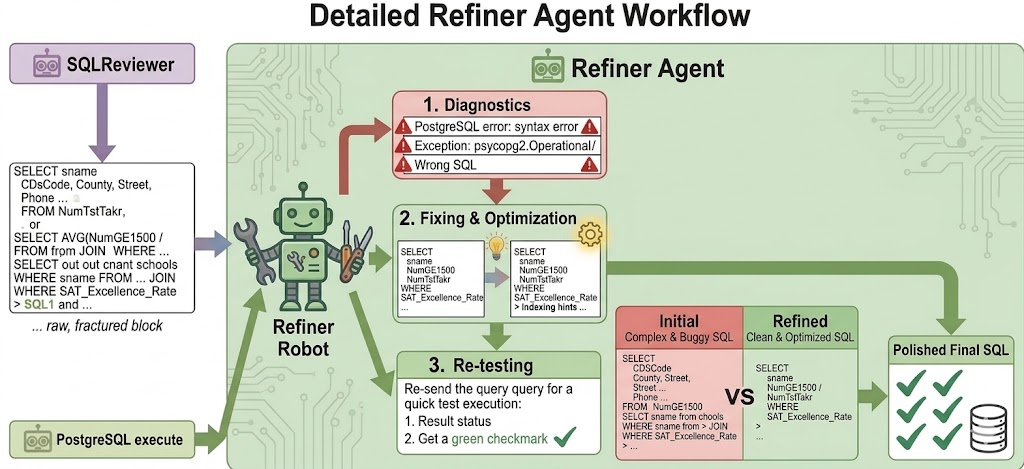
\includegraphics[width=\linewidth,height=0.9\textheight,keepaspectratio]{images/ai/Refiner.jpeg}
    \caption{The Refiner}
    \label{fig:The Refiner}
\end{figure}

The Refiner agent operates as a correction and refinement layer. It receives:

\begin{itemize}
    \item The generated SQL from the Decomposer
    \item The SQL Reviewer's validation report (if available)
    \item The original database schema
    \item The original natural language question
    \item Optionally, error messages from a previous failed execution attempt
\end{itemize}

The Refiner's role is to:

\begin{enumerate}
    \item Address issues identified by the SQL Reviewer (syntax errors, type mismatches, missing JOINs)
    \item Detect logical errors in the SQL (e.g., incorrect aggregation semantics)
    \item Correct PostgreSQL-specific issues
    \item Ensure the query aligns with the user's intent
    \item If provided with an execution error, diagnose and fix the cause
\end{enumerate}

This iterative refinement approach handles the common case where initial generation produces syntactically valid but semantically incorrect SQL. Rather than failing immediately, the Refiner attempts correction, improving overall success rates.

\subsection{Agent Prompting and In-Context Learning}

Prompt engineering and in-context learning are central to the system's robustness. Each agent receives a carefully constructed prompt that combines (1) a \textit{system} instruction describing the agent role and constraints, (2) structured context (schema JSON, sample values), and (3) zero- or few-shot examples demonstrating the expected output format. Prompts enforce structured outputs (JSON or clearly delimited SQL blocks) and rely on deterministic settings for validation steps while allowing modest stochasticity for creative decomposition.

\subsubsection{Selector: Retrieval-Augmented, Few-Shot Prompts}

The Selector uses a retrieval-augmented prompt. The prompt contains a compact JSON representation of the full schema, several short few-shot examples mapping questions to relevant tables/columns, and an explicit instruction to return a small curated schema subset in JSON. For reliability the Selector runs with a low temperature (e.g., 0.0--0.2) and explicit parsing instructions so downstream components can consume its output deterministically.

\subsubsection{Decomposer: Chain-of-Thought (Structured) Prompts}

The Decomposer employs chain-of-thought style prompting expressed in a structured template. Prompts include one-shot or few-shot demonstrations showing how to decompose a complex natural-language question into numbered sub-questions and matching intermediate SQL fragments. The prompt asks the model to output a JSON object with fields: \texttt{subquestions}, \texttt{intermediate\_sql}, and \texttt{final\_sql}. Temperature is kept moderate (e.g., 0.2--0.4) to allow reasoning while keeping outputs stable.

\subsubsection{SQL Reviewer: Rule-driven, Deterministic Prompts}

The SQL Reviewer receives rule-driven prompts acting as a checklist. The prompt emphasizes PostgreSQL syntax rules, schema presence checks, and type compatibility tests. The model is instructed to return a structured report: a pass/fail flag and a list of named issues (column not found, type mismatch, missing JOIN, suspicious predicate, etc.). The Reviewer is run with deterministic decoding (temperature = 0) and strict output formatting so the service can parse and act on findings automatically.

\subsubsection{Refiner: Error-driven Iterative Prompts}

The Refiner uses iterative, error-driven prompting. Its prompt includes: the original question, the curated schema, the Decomposer's SQL, the SQL Reviewer's report, and, when applicable, the database execution error message. In-context examples show how to transform an erroneous SQL into a corrected form and how to explain the correction succinctly. The Refiner returns corrected SQL (and an optional brief rationale) in a structured format; temperature is low to moderate to favor corrective precision.

\subsubsection{Structured Prompting and Output Enforcement}

Across all agents the prompts enforce a machine-parseable output format (JSON, fenced SQL blocks) to avoid hallucinated or ambiguous text. The service uses small parsing helpers (see \texttt{core.utils.parse\_json}) to validate model outputs and fall back to conservative repairs when parsing fails. When available, the system uses LLM "function-calling" or equivalent structured-output features to further reduce parsing errors.

\subsubsection{In-Context Learning Strategy}

In-context learning is applied selectively: few-shot examples are chosen from the \texttt{mini\_dev} BIRD subset and from historical platform queries, selected by semantic similarity to the target question. Dataset-specific templates (the BIRD \texttt{mini\_dev} templates) are injected as examples for the Decomposer and Refiner. This approach provides strong, task-relevant inductive bias without full fine-tuning and enables the model to adapt to domain-specific naming conventions discovered during the SQLite→PostgreSQL migration.

\subsection{Implementation Details}

\subsubsection{Service Entry Point and Configuration}

The text-to-SQL service is implemented as a FastAPI application in Python. The service is configurable via environment variables:

\begin{itemize}
    \item \texttt{LLM\_API\_KEY}: Authentication token for the LLM provider (required)
    \item \texttt{LLM\_MODEL}: Model identifier (defaults to \texttt{gpt-4o})
    \item \texttt{LLM\_API\_BASE}: API endpoint URL (defaults to GitHub's model inference service)
\end{itemize}

The \texttt{AgentService} class wraps the multi-agent pipeline and provides a unified interface to the FastAPI application. Upon initialization, the service validates that an API key is provided and configures the OpenAI client with the specified endpoint. Configuration is performed once during startup via the singleton pattern, avoiding repeated LLM client initialization.

\subsubsection{Schema Extraction and Representation}

For each database, the service constructs a normalized schema representation containing:

\begin{itemize}
    \item Table names and their purposes (extracted from database comments if available)
    \item Column names, data types, and nullability constraints
    \item Foreign key relationships between tables
    \item Sample values from each column (limited to a few rows to maintain token efficiency)
    \item Primary key and unique constraint information
\end{itemize}

This schema representation is formatted as structured JSON and passed to the Selector agent as context. The JSON format allows the LLM to parse schema information precisely, reducing hallucination of non-existent tables or columns.

\subsubsection{Agent Communication Protocol}

Each agent is implemented as a Python class inheriting from a \texttt{BaseAgent} interface. The agents communicate via a message-passing protocol:

\begin{itemize}
    \item Each agent implements a \texttt{talk(message: dict)} method
    \item Messages contain the question, database schema, previous reasoning, and execution results
    \item Agents return their reasoning process and generated output (e.g., SQL statements)
    \item The reasoning is logged and can be used for debugging or audit trails
\end{itemize}

This message-passing architecture makes the pipeline transparent: the complete reasoning chain of all four agents is preserved for inspection, supporting debugging of incorrect query generation and providing explainability to users.

\subsubsection{Error Handling and Iterative Refinement}

When a generated SQL query fails validation/execution in the Reviewer stage (e.g., due to a column name typo, missing JOIN, or semantic mismatch with the question), the service implements an iterative refinement loop:

\begin{enumerate}
    \item The Decomposer generates initial SQL
    \item The SQL Reviewer validates semantics and attempts controlled execution
    \item If validation fails or execution fails, the Reviewer's error message and reasoning are captured
    \item The Refiner is invoked with the Reviewer's diagnostics
    \item The Refiner suggests corrections
    \item The SQL Reviewer re-validates and re-attempts execution with the corrected query
\end{enumerate}

This loop can execute up to a configured maximum number of iterations, preventing infinite loops while allowing transient issues to be resolved. Successful queries are cached to avoid regeneration for identical or highly similar questions.

\subsection{Deployment Architecture}

\subsubsection{Containerization}

The text-to-SQL service is containerized using Docker for consistent deployment across environments. The Dockerfile employs a multi-stage build:

\begin{enumerate}
    \item \textit{Build stage}: Installs Python dependencies and prepares the service code
    \item \textit{Runtime stage}: Includes only runtime dependencies (psycopg2 client libraries, Python runtime) and the service code, minimizing image size
\end{enumerate}

The Docker image is configured to start the service via a shell script (\texttt{start.sh}) that:

\begin{itemize}
    \item Validates required environment variables
    \item Waits for the LLM API endpoint to become available (if using remote inference)
    \item Launches the FastAPI server on a configurable port (default: 8000)
\end{itemize}

\subsubsection{Kubernetes Deployment}

In production, the text-to-SQL service is deployed to Kubernetes as a \texttt{Deployment} resource. Key configuration decisions:

\begin{itemize}
    \item \textbf{Replica count}: 2--3 replicas ensure availability and support rolling updates
    \item \textbf{Resource requests}: CPU and memory requests are set conservatively to prevent resource contention with other cluster services
    \item \textbf{Liveness and readiness probes}: HTTP probes verify that the service is healthy and ready to accept requests
    \item \textbf{Environment variables}: LLM configuration is passed via Kubernetes Secrets to avoid hardcoding credentials
\end{itemize}

A Kubernetes Service exposes the deployment internally to the backend via DNS. Optionally, an Ingress resource can route external traffic to the service for testing or public API scenarios.

\subsection{Performance Optimization}

\subsubsection{Token Budget Management}

LLM API costs and latency are proportional to token count. The service implements several optimizations:

\begin{enumerate}
    \item \textbf{Schema filtering}: The Selector eliminates irrelevant tables before passing schema to the Decomposer, reducing schema context in typical cases
    \item \textbf{Structured prompts}: Prompts use JSON schemas and explicit formatting instructions rather than free-form text, improving parsing reliability and reducing redundant token usage
    \item \textbf{Caching}: Frequently asked questions over stable schemas are cached, avoiding re-generation
    \item \textbf{Batch processing}: For evaluation datasets, the service supports batch inference, amortizing API connection overhead
\end{enumerate}

\subsection{Evaluation and Quality Metrics}

The text-to-SQL service is evaluated on a subset of the BIRD benchmark dataset. The standard BIRD dataset was originally provided in SQLite format; to align with the PostgreSQL-centric design of the platform, the dataset was migrated from SQLite to PostgreSQL. Due to schema complexity and migration constraints, a curated subset (denoted \texttt{mini\_dev}) was used for evaluation, containing representative queries across multiple complexity levels and database domains.

Evaluation metrics include:

\begin{enumerate}
    \item \textbf{Execution Accuracy (EX)}: The percentage of generated queries that produce the same result as the ground-truth query, even if the SQL text differs. This metric captures semantic correctness:
    \[\text{EX} = \frac{\text{Number of queries with matching execution results}}{\text{Total number of queries}} \times 100\%\]
    
    \item \textbf{Valid Efficiency Score (VES)}: the execution efficiency of generated SQL queries relative to gold-standard queries, but only for queries that return correct results. It rewards queries that are both correct and faster than the reference:    
    \begin{itemize}
      \item Per-Query Execution Time Ratio:
         \begin{equation}
            R_i = \frac{1}{|M_i|} \sum_{j \in M_i} \frac{T_{\text{gold}, j}}{T_{\text{pred}, j}}
         \end{equation}
         \begin{itemize}
            \item $T_{\text{gold}, j}$ is the execution time of the ground-truth SQL query during iteration $j$.
            \item $T_{\text{pred}, j}$ is the execution time of the predicted SQL query during iteration $j$.
            \item $M_i$ represents the filtered subset of stable iterations following outlier removal.
         \end{itemize}
      \item Dataset-Wide VES Calculation:
         \begin{equation}
            \text{VES} = \frac{1}{Q} \sum_{i=1}^{Q} \left( \sqrt{R_i} \times 100 \right)
         \end{equation}
         \begin{itemize}
            \item $Q$ is the total number of evaluation instances (queries) in the benchmark dataset.
            \item $R_i$ is the execution time ratio computed for the $i$-th query.
         \end{itemize}
        \item $\text{VES} = 100 \implies$ generated SQL is equally efficient as gold SQL
        \item $\text{VES} > 100 \implies$ generated SQL is faster than gold SQL
        \item $\text{VES} < 100 \implies$ generated SQL is slower than gold SQL
   \end{itemize}
\end{enumerate}

Performance varies by question complexity:

\begin{table}[h]
    \centering
    \begin{tabular}{lcccc}
        \toprule
        \textbf{Metric} & \textbf{Simple} & \textbf{Moderate} & \textbf{Challenging} & \textbf{Total} \\
        \midrule
        Query Count      & 62       & 47        & 39        & 148  \\
        Passed Queries   & 42       & 27        & 23        & 92  \\
        Mismatches       & 20       & 20        & 16        & 56   \\
        EX Accuracy (\%) & 67.74    & 57.45     & 58.97     & 62.16 \\
        VES Score (\%)   & 70.47    & 55.75     & 59.53     & 62.91 \\
        \bottomrule
    \end{tabular}
    \caption{Text-to-SQL Service Performance by Query Complexity: Query distribution across complexity categories with detailed breakdown of passed queries, mismatches, and Execution Accuracy (EX) and Value Equivalence Score (VES) metrics.}
    \label{tab:text_to_sql_performance}
\end{table}

This degradation in moderate-complexity queries reflects the fundamental challenge of mapping natural language ambiguity to precise SQL semantics. The recovery in challenging queries suggests that the multi-agent pipeline's error correction mechanisms are particularly effective for more complex scenarios where explicit decomposition provides substantial benefit.

\subsection{Integration with the Backend}

The backend exposes a \texttt{/text-to-sql/generate} endpoint that:

\begin{enumerate}
    \item Validates that the authenticated user has access to the specified project
    \item Extracts database connection credentials from the project configuration
    \item Forwards the request to the text-to-SQL service
    \item Receives the generated SQL from the service
    \item Executes the SQL through the standard query execution pipeline
    \item Returns results or errors to the user
\end{enumerate}

This integration ensures that text-to-SQL queries inherit all backend security controls (row-level access policies, audit logging, transaction isolation) as if they were manually written SQL queries.

\subsection{Limitations and Future Work}

Current limitations of the text-to-SQL service include:

\begin{itemize}
    \item \textbf{Context length}: Schemas exceeding LLM context limits (typically 100k tokens) cannot be fully represented, requiring manual schema curation
    \item \textbf{Ambiguity}: Natural language questions with multiple valid SQL interpretations may generate incorrect queries without explicit user hints
    \item \textbf{Domain-specific syntax}: Database-specific features (e.g., PostgreSQL window functions, temporal queries) require additional in-context examples
    \item \textbf{Latency}: Multi-agent generation introduces 2--8 second latency, unsuitable for real-time interactive dashboards
\end{itemize}

Future improvements include:

\begin{enumerate}
    \item \textbf{Fine-tuning}: Training smaller, domain-specific models on the platform's historical queries to reduce cost and latency
    \item \textbf{Interactive refinement}: Allowing users to provide feedback on incorrect queries, which the Refiner uses to improve subsequent generations
    \item \textbf{Intermediate verification}: Running intermediate queries from the Decomposer to verify they produce sensible results before proceeding to final SQL
    \item \textbf{Federated schema support}: Extending the service to generate queries joining tables across multiple databases
\end{enumerate}
